
The character controlled by the player is CatBot: a robot that looks like the cat, that has a failing control system that constants needs fixing. A cat was chosen as a combination for a few reasons. First, the developer is good, and enjoys, drawing cats. Second, cats are popular companions with an estimated 10.2 million pet cats in the UK \citep{CatOwnership}. And, finally, but more importantly, the developer had an existing sprite-sheet, shown in  that could be re-used, alongside an existing system that could be used as a base.

\begin{figure}
    \centering
    \begin{subfigure}[t]{0.45\linewidth}
        \centering
        
\includegraphics[width=1\linewidth]{C5/CatBot/Jumping.png}
        \caption{CatBot jumping}
    \end{subfigure}
    \begin{subfigure}[t]{0.45\linewidth}
        \centering
        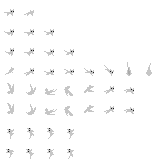
\includegraphics[width=0.75\linewidth]{C5/CatBot/SpriteSheet.png}
        \caption{Sprite-sheet}
    \end{subfigure}
    \caption[CatBot and CatBot's sprite-sheet]{CatBot and CatBot's sprite-sheet, available in \texttt{res://assets/player/Kitis.png}. Only rows 1 -- 4 were used for CatBot.}
    \label{fig:design/catBotSpriteSheet}
\end{figure}

CatBot (found in \texttt{res://src/entities/player/player\_cat.tcsn}), which extends the custom-made \texttt{generic\_entity} class (...\texttt{/classes/generic\_entity.gd}). \texttt{generic\_entity} provides basic functions such managing HP, stability, and typing\footnote{Godot default type methods only provide the node type. Providing this method as a base to all entities makes implementing future systems easier}; and, in turn, extends the built-in \href{https://docs.godotengine.org/en/stable/classes/class\_characterbody2d.html}{Character Body 2D} node, which is designed \textquote{for physics bodies that are meant to be user-controlled}. This provides numerous functions, such as \texttt{move\_and\_slide()}, and attributes such as \texttt{velocity}.

The structure of the CatBot scene is shown in \autoref{fig:design/catBot-NodeStructure}. A summary of the mechanics chosen are shown in \autoref{sec:design/CatBot/ability}. CatBot was initially designed as a traditional platformer character, summarised in \autoref{sec:design/CatBot/traditional}, and then adapted to remove the controls, detailed in \autoref{sec:design/CatBot/modularisation}. Finally, CatCode was developed, the basics of how these systems interact with CatBot are shown in \autoref{sec:design/CatBot/instancing}.

\begin{figure}
    \centering
    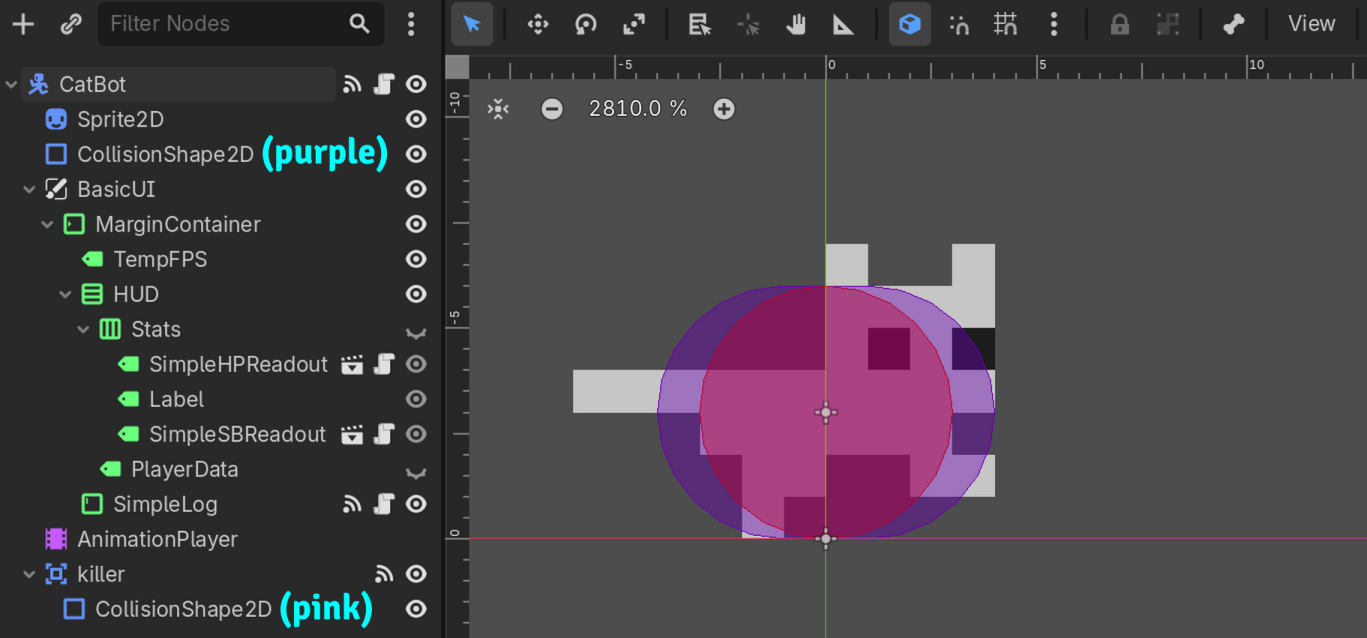
\includegraphics[width=0.75\linewidth]{C5//CatBot/nodeStructure.png}
    \caption[CatBot node structure]{CatBot node structure}
    \label{fig:design/catBot-NodeStructure}
\end{figure}

\subsection{Mechanics}\label{sec:design/CatBot/ability}

\paragraph{Horizontal Movement}

Horizontal movement is handelled by adding \texttt{SPEED * direction * delta} to \texttt{velocity.x}, where \texttt{delta} is the time since last frame, \texttt{direction} is the horizontal input where 1 is right, and -1 is left, and \texttt{SPEED} is a constant determined through two other constants \texttt{MAX\_SPEED} and \texttt{SLIPMOD} (which controls \textquote{slippiness})

\begin{figure}
    \begin{fullwidth}
    \begin{tcolorbox}[boxrule=0.25mm]
    \begin{verbatim}
## Handles horizontal physics
func horizontal_physics(_delta: float, direction: float) -> void:
    var slipmod_adjustment := 1.0 if abs(direction) > 0 else SLIPMOD*0.75
    velocity.x = lerp(velocity.x, 0.0, FRICTION_CONST * slipmod_adjustment)
    \end{verbatim}
    \end{tcolorbox}
    \end{fullwidth}
    \caption{Horizontal physics function}
    \label{fig:design/catBot-HorPhys}
\end{figure}

Friction is more complex, using the \texttt{lerp()} function to allow for a non-linear regression in momentum whilst remaining consistent at different frame-rates. The constant \texttt{FRICTION\_CONST} is used to determine the strength of the friction, as well as \texttt{SLIPMOD} when not running. This is handled by the function in \autoref{fig:design/catBot-HorPhys}.

\paragraph{Vertical Physics and Jumping}

Every frame \texttt{is\_on\_floor()} is false (meaning CatBot is in the air), the global gravity value (gotten using the method \texttt{get\_gravity()}) is \textit{added} to \texttt{velocity.y}\footnote{The y-axis is inverted in Godot's 2D engine.}. When this is true, \texttt{air\_time()} is increased by \texttt{delta}.

To jump, we set \texttt{velocity.y} to \texttt{JUMP\_VELOCITY} if grounded. For the purposes of jumping, to improve the feel of movement, we have implemented Coyote inspired by \textbf{[Celeste TODO]}. This changed the condition to jump from \texttt{is\_on\_floor()} to \texttt{air\_time < COYOTE\_TIME}.

\subsection{Traditional Systems}\label{sec:design/CatBot/traditional}

\subsection{Extracting the Controllers}\label{sec:design/CatBot/modularisation}

\subsection{Instancing CatBot}\label{sec:design/CatBot/instancing}
